
\begin{figure}[htbp]
	\hspace{-1.9cm}
	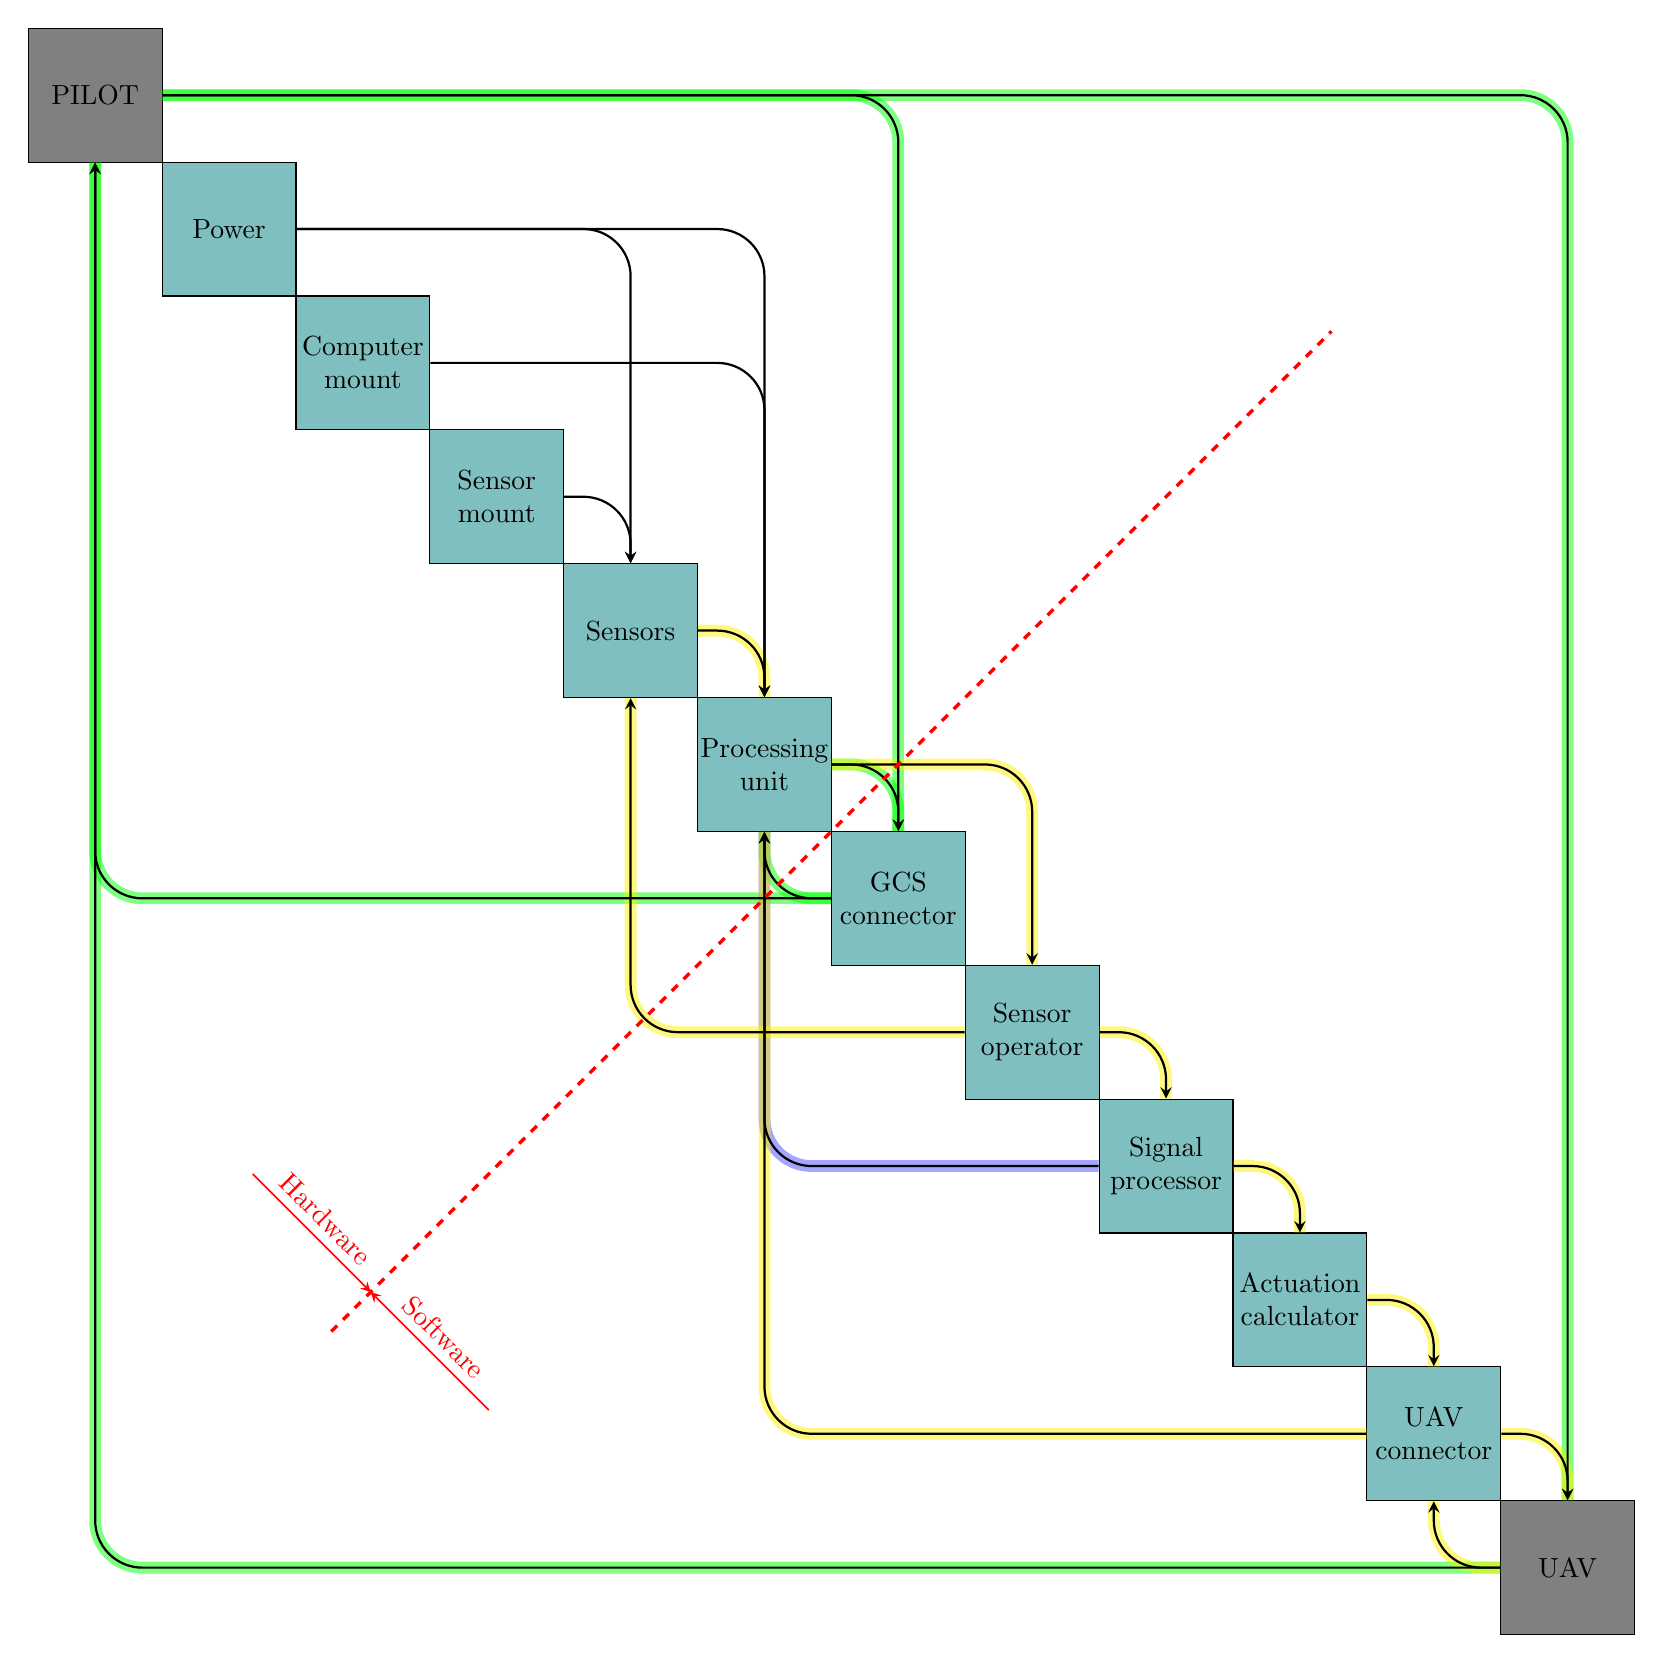
\begin{tikzpicture}

		\tikzstyle{module}=[rectangle,
			fill=teal!50,draw=black,
			minimum height=1.7cm,minimum width=1.7cm,
			node distance=2.4042cm,	%=sqrt(1.7cm)
			align=center,inner sep=0mm]
		\tikzstyle{arrow}=[->,>=stealth,
			draw=black,thick,
			rounded corners=0.6cm]
		\tikzstyle{shadow}=[
			draw=black,opacity=0.5,line width=1.5mm,
			rounded corners=0.6cm]

		\node[module,fill=gray]	(pilot)	{PILOT};
		\node[module,below right of=pilot]	(power)	{Power};
		\node[module,below right of=power]	(computer-m)	{Computer\\ mount};
		\node[module,below right of=computer-m]	(sensor-m)	{Sensor\\ mount};
		\node[module,below right of=sensor-m]	(sensors)	{Sensors};
		\node[module,below right of=sensors]	(cpu)	{Processing\\ unit};
		\node[module,below right of=cpu]	(gcs)	{GCS\\ connector};
		\node[module,below right of=gcs]	(sensor-o)	{Sensor\\ operator};
		\node[module,below right of=sensor-o]	(signal)	{Signal\\ processor};
		\node[module,below right of=signal]	(actuation)	{Actuation\\ calculator};
		\node[module,below right of=actuation]	(uav)	{UAV\\ connector};
		\node[module,below right of=uav,fill=gray]	(UAV)	{UAV};


			\draw[shadow,draw=green]	(pilot)		-|	(gcs);
			\draw[shadow,draw=green]	(pilot)		-|	(UAV);
			\draw[shadow,draw=green]	(UAV)		-|	(pilot);
			\draw[shadow,draw=green]	(gcs)		-|	(pilot);
			\draw[shadow,draw=yellow]	(sensors)	-|	(cpu);
			\draw[shadow,draw=green]	(cpu)		-|	(gcs);
			\draw[shadow,draw=green]	(gcs)		-|	(cpu);
			\draw[shadow,draw=yellow]	(cpu)		-|	(sensor-o);
			\draw[shadow,draw=blue!70]	(signal)		-|	(cpu);
			\draw[shadow,draw=yellow]	(uav)		-|	(cpu);
			\draw[shadow,draw=yellow]	(sensor-o)	-|	(signal);
			\draw[shadow,draw=yellow]	(sensor-o)	-|	(sensors);
			\draw[shadow,draw=yellow]	(signal)	-|	(actuation);
			\draw[shadow,draw=yellow]	(actuation)	-|	(uav);
			\draw[shadow,draw=yellow]	(uav)		-|	(UAV);
			\draw[shadow,draw=yellow]	(UAV)		-|	(uav);
		
		\draw[arrow]	(pilot)		-|	(gcs);
		\draw[arrow]	(pilot)		-|	(UAV);
		\draw[arrow]	(UAV)		-|	(pilot);
		\draw[arrow]	(gcs)		-|	(pilot);

		\draw[arrow]	(power)		-|	(sensors);
		\draw[arrow]	(power)		-|	(cpu);

		\draw[arrow]	(computer-m)-|	(cpu);

		\draw[arrow]	(sensor-m)	-|	(sensors);

		\draw[arrow]	(sensors)	-|	(cpu);

		\draw[arrow]	(cpu)		-|	(gcs);
		\draw[arrow]	(gcs)		-|	(cpu);
		\draw[arrow]	(cpu)		-|	(sensor-o);
		\draw[arrow]	(signal)	-|	(cpu);
		\draw[arrow]	(uav)		-|	(cpu);

		\draw[arrow]	(sensor-o)	-|	(signal);
		\draw[arrow]	(sensor-o)	-|	(sensors);

		\draw[arrow]	(signal)	-|	(actuation);

		\draw[arrow]	(actuation)	-|	(uav);

		\draw[arrow]	(uav)		-|	(UAV);
		\draw[arrow]	(UAV)		-|	(uav);


		\draw[red,very thick,dashed]	(3,-15.7) -- (15.7,-3);
		\draw[red,->,>=stealth,semithick]	(2,-13.7) -- node[sloped,anchor=south]{Hardware} (3.5,-15.2);
		\draw[red,<-,>=stealth,semithick]	(3.5,-15.2) -- node[sloped,anchor=south]{Software} (5,-16.7);

	\end{tikzpicture}

	\caption{OCAS N$^2$ diagram for interfaces definition}
	\label{fig:N2}
\end{figure}
